%% Models
%%=========================================

\chapter{Models}
\label{ch:models}
In this chapter we present the three models we created during our iterative development process. We present the {\tt VecRep} model in Section \ref{sec:repeat_vector}, and our two encoder-decoder based models {\tt EncDecReg} and {\tt EncDecAtt} are presented in Sections \ref{sec:regular_encoder_decoder} and \ref{sec:attention_encoder_decoder}.

%%=========================================

\section{Repeat Vector}
\label{sec:repeat_vector}
The first model, called {\tt VecRep} for short, has a similar structure to that of the encoder-decoder framework. This model consists of two groups of LSTMs. The first group reads the entire input and outputs its value from the last iteration. This output is then repeated in the dimension of time, and inputted into a new group of LSTMs.

\begin{figure}[ht]
    \centering
    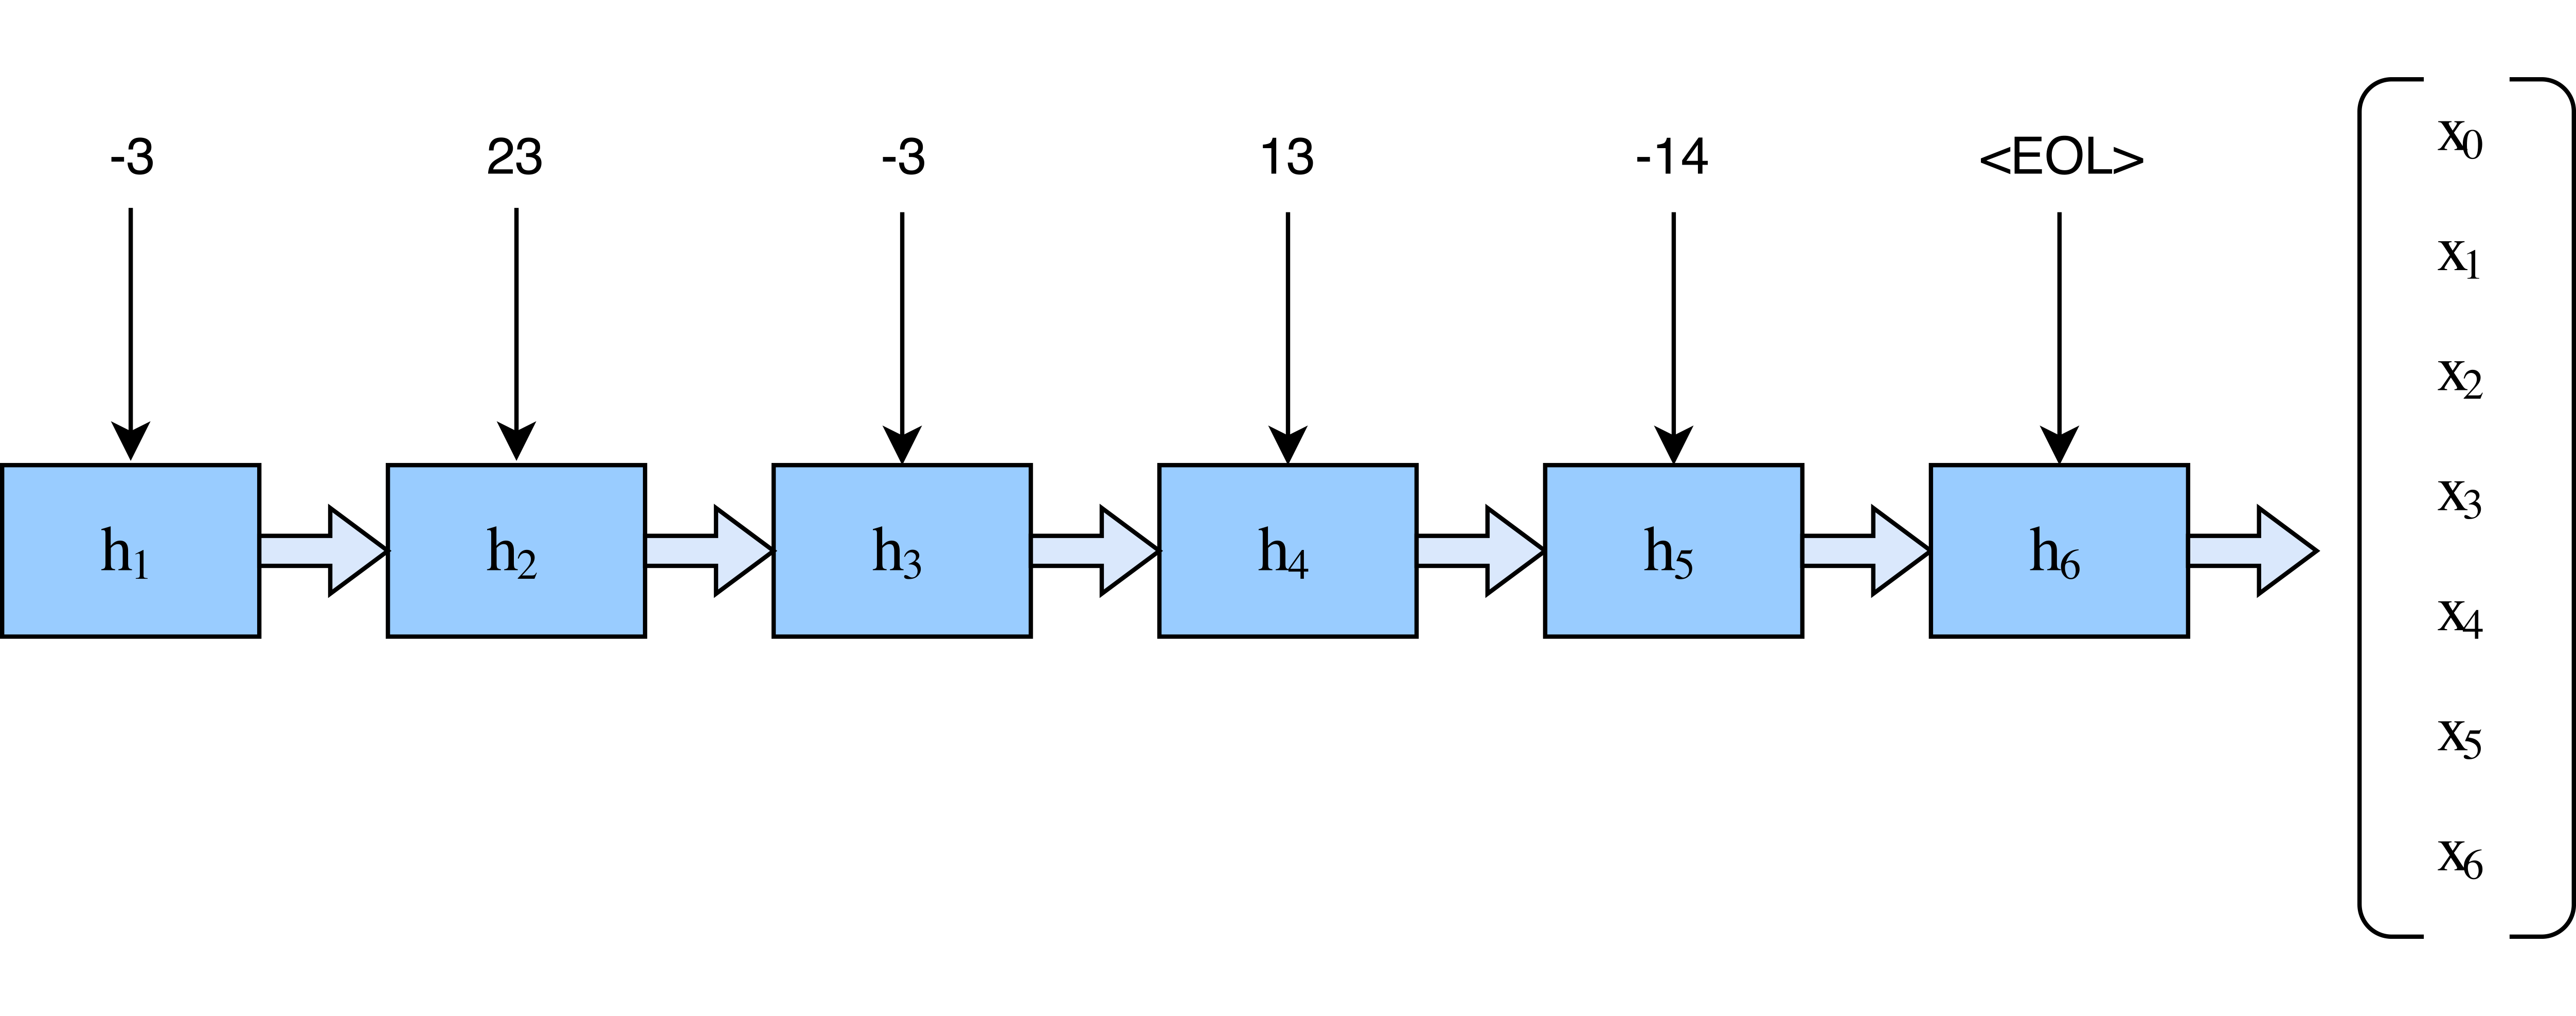
\includegraphics[width=0.7\textwidth]{fig/development_process/lstm-vector-projection-encoder.png}
    \caption{A LSTM outputting its final hidden state after reading a sequence}
    \label{fig:lstm-vector-projection-encoder}
\end{figure}

Figure \ref{fig:lstm-vector-projection-encoder} illustrates a regular LSTM that reads an input sequence and output the values from the last iteration. The output vector has a length equal to the number of units in the LSTM. As illustrated in Figure \ref{fig:lstm-vector-projection-decoder}, the output from the LSTM is repeated \(N\) times, where \(N\) is the length of the output sequence. This means we take an output shape of {\tt (units)} from the first group of LSTMs, and turn it into a shape of {\tt (N, units)}.

\begin{figure}[ht]
    \centering
    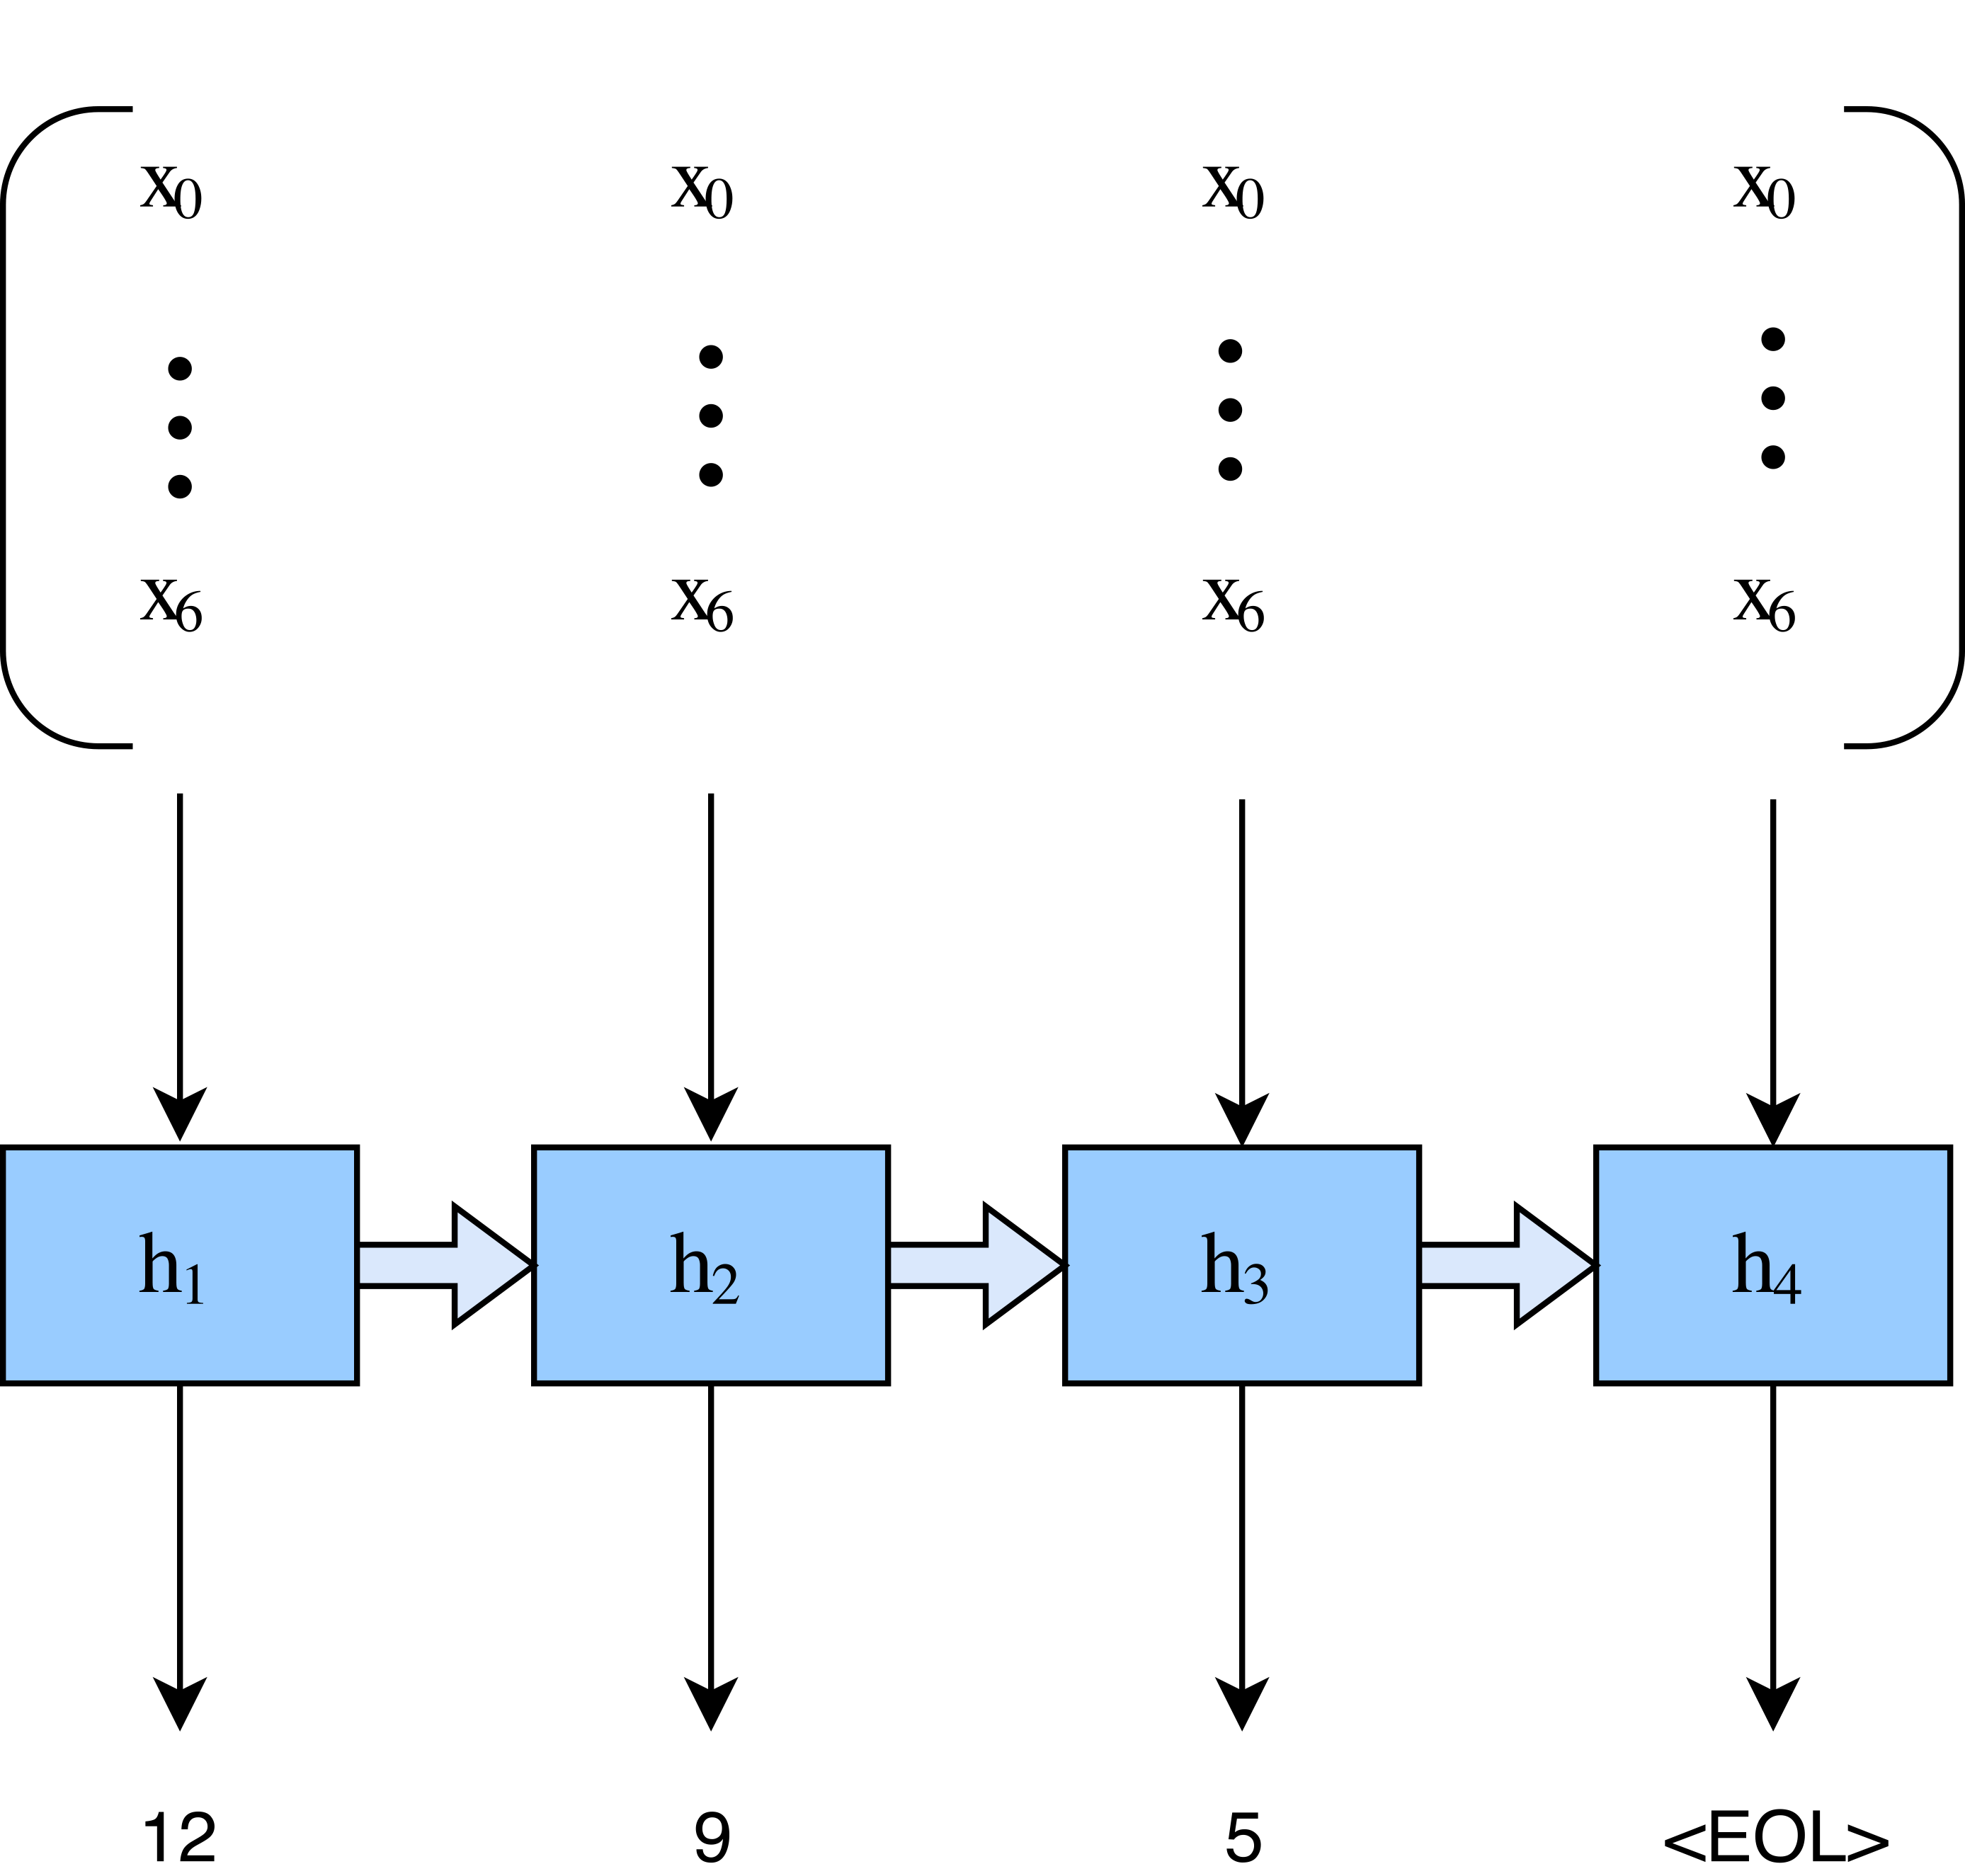
\includegraphics[width=0.5\textwidth]{fig/development_process/lstm-vector-projection-decoder.png}
    \caption{Repeating the output from a LSTM and feeding it to another LSTM}
    \label{fig:lstm-vector-projection-decoder}
\end{figure}

In this example, the output has a length of three characters, plus a special ``end of line'' character, which means the repeated matrix has a size of \(4, u\), where \(u\) is the number of units in the LSTM cell. The resulting matrix of the repeated vector is then fed to another LSTM that reads each time step and outputs for each iteration.

\begin{figure}[!ht]
    \centering
    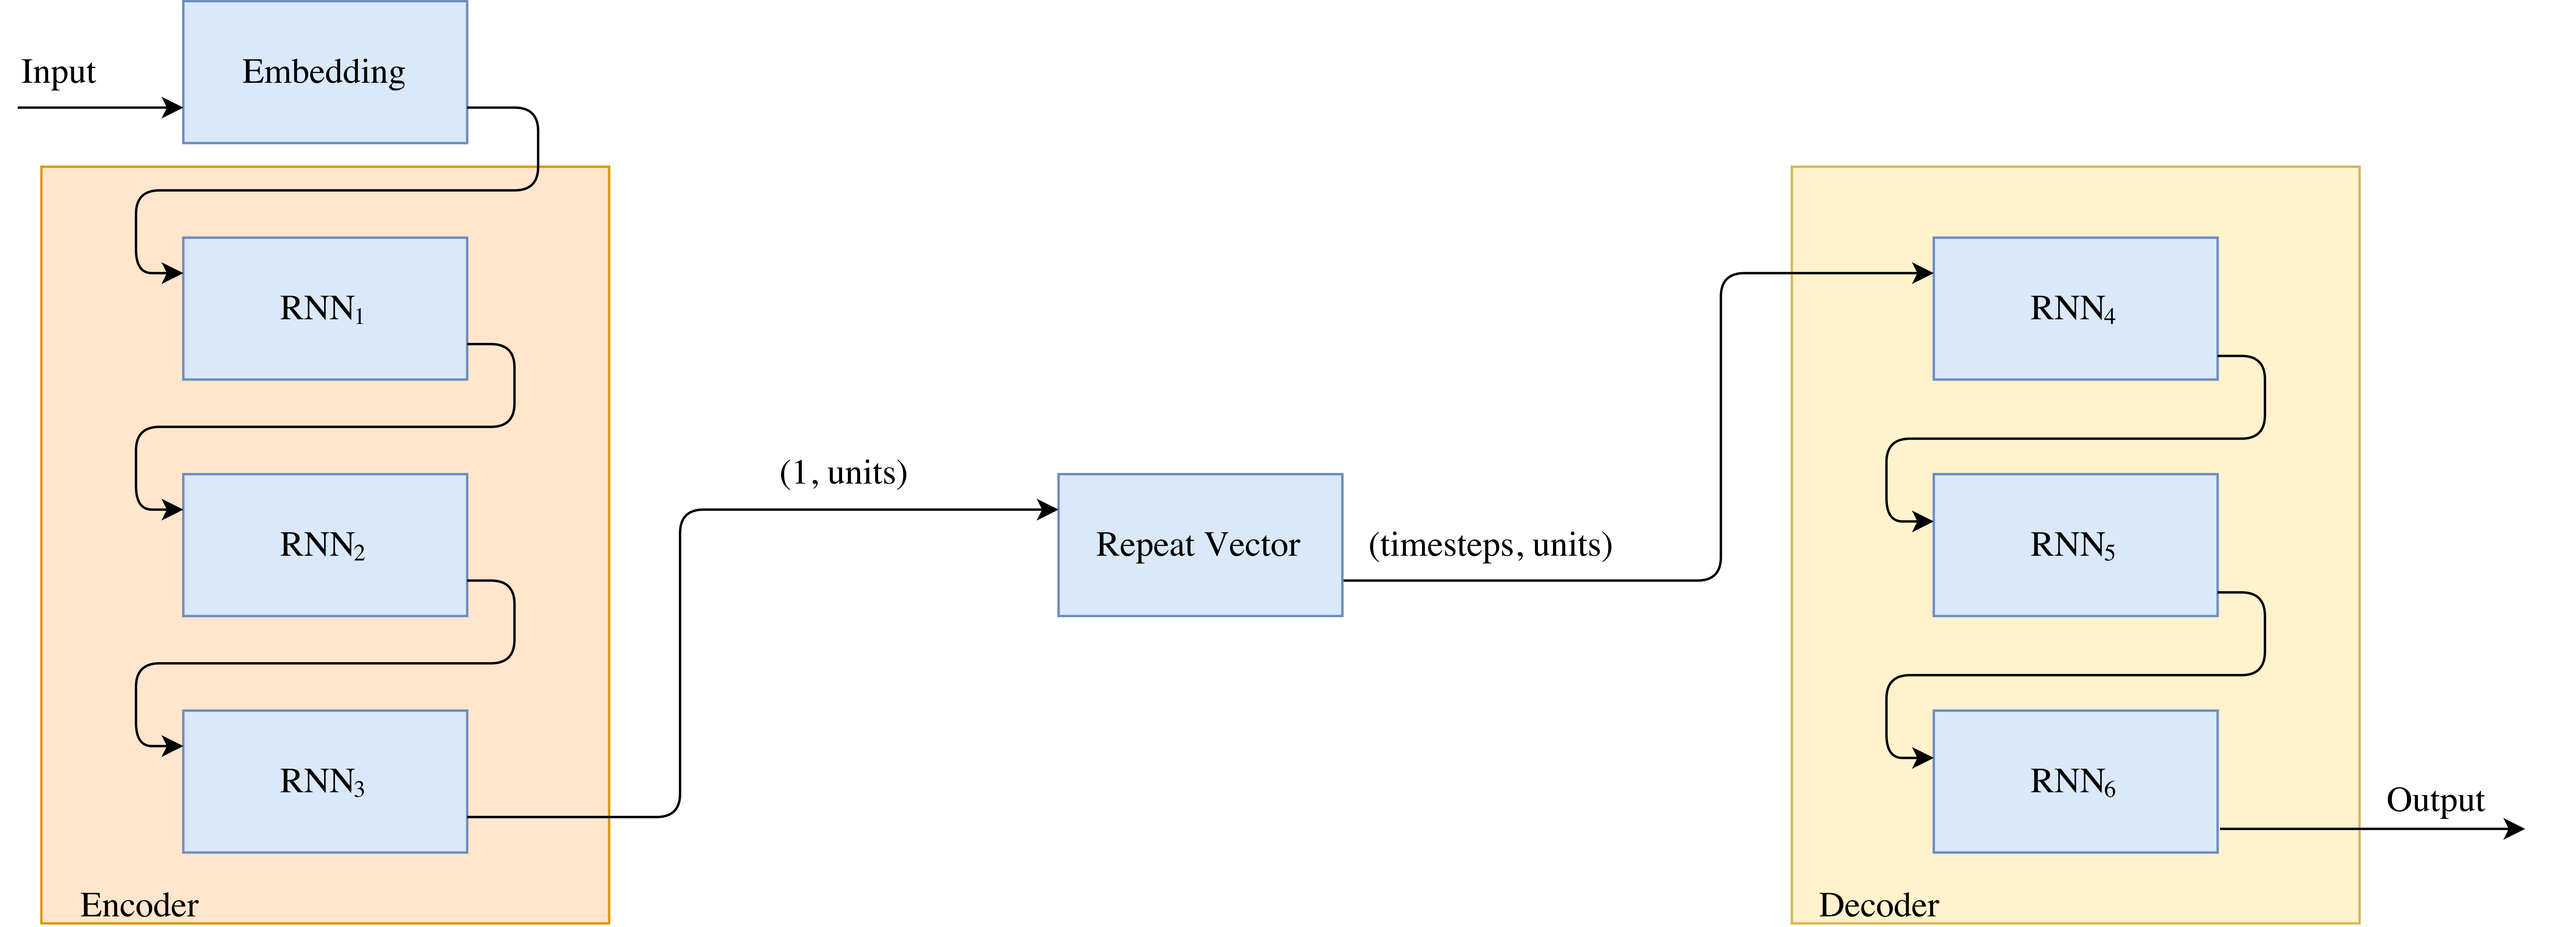
\includegraphics[width=1\textwidth]{fig/models/vecrep_model.png}
    \caption{Simplified illustration of the {\tt VecRep} model}
    \label{fig:vecrep_model}
\end{figure}

The {\tt VecRep} model is illustrated in Figure \ref{fig:vecrep_model}. The ``encoder'' and ``decoder'' both consists of three recurrent units. These units are stacked sequentially, which means that the first cell, \(\text{RNN'}_1\) completed all its iterations, and the output from this cell is then fed to the next RNN cell which does the same. The recurrent cells that are marked, such as \(\text{RNN'}_1\), indicates that the cell returns its output for every iteration, whereas a cell that is not marked only outputs from the last iteration. The ``encoding'' in this model is done by the \(\text{RNN}_3\) cell, which only outputs in the last iteration, an approach that is similar to the encoded context vector in the encoder-decoder framework. Between the two stacks of recurrent units is the layer which repeats the final output of \(\text{RNN}_3\) in the dimension of time for the first unit in the decoder.

%%=========================================

\section{Regular Encoder-Decoder}
\label{sec:regular_encoder_decoder}
The second model implements the encoder-decoder framework. It is called {\tt EncDecReg} as it is the ``regular'' encoder-decoder, unlike the last model. This model has certain similarities to the {\tt VecRep} model; also this one consists of two groups of LSTMs, where the first group encodes the input and the last group decodes.

However, in this model, we use the last hidden state of the encoder, instead of the output as with the {\tt VecRep} model. In addition, during testing and validation, the decoder feed its output back in as input. However, feeding the output back as input is not used during training, where we use the actual labels instead. This is similar to the approach taken by \cite{bengio2015scheduled}.

This model also uses two embeddings, one for the input and one for the output. The input is embedded before the encoder reads the input, and the output embedding is applied on the fly when the decoder is reusing its output as input. This is in contrast to the {\tt VecRep} model which only used embedding for the input data. Both the embeddings in this model is fully trainable.

\begin{figure}[!ht]
    \centering
    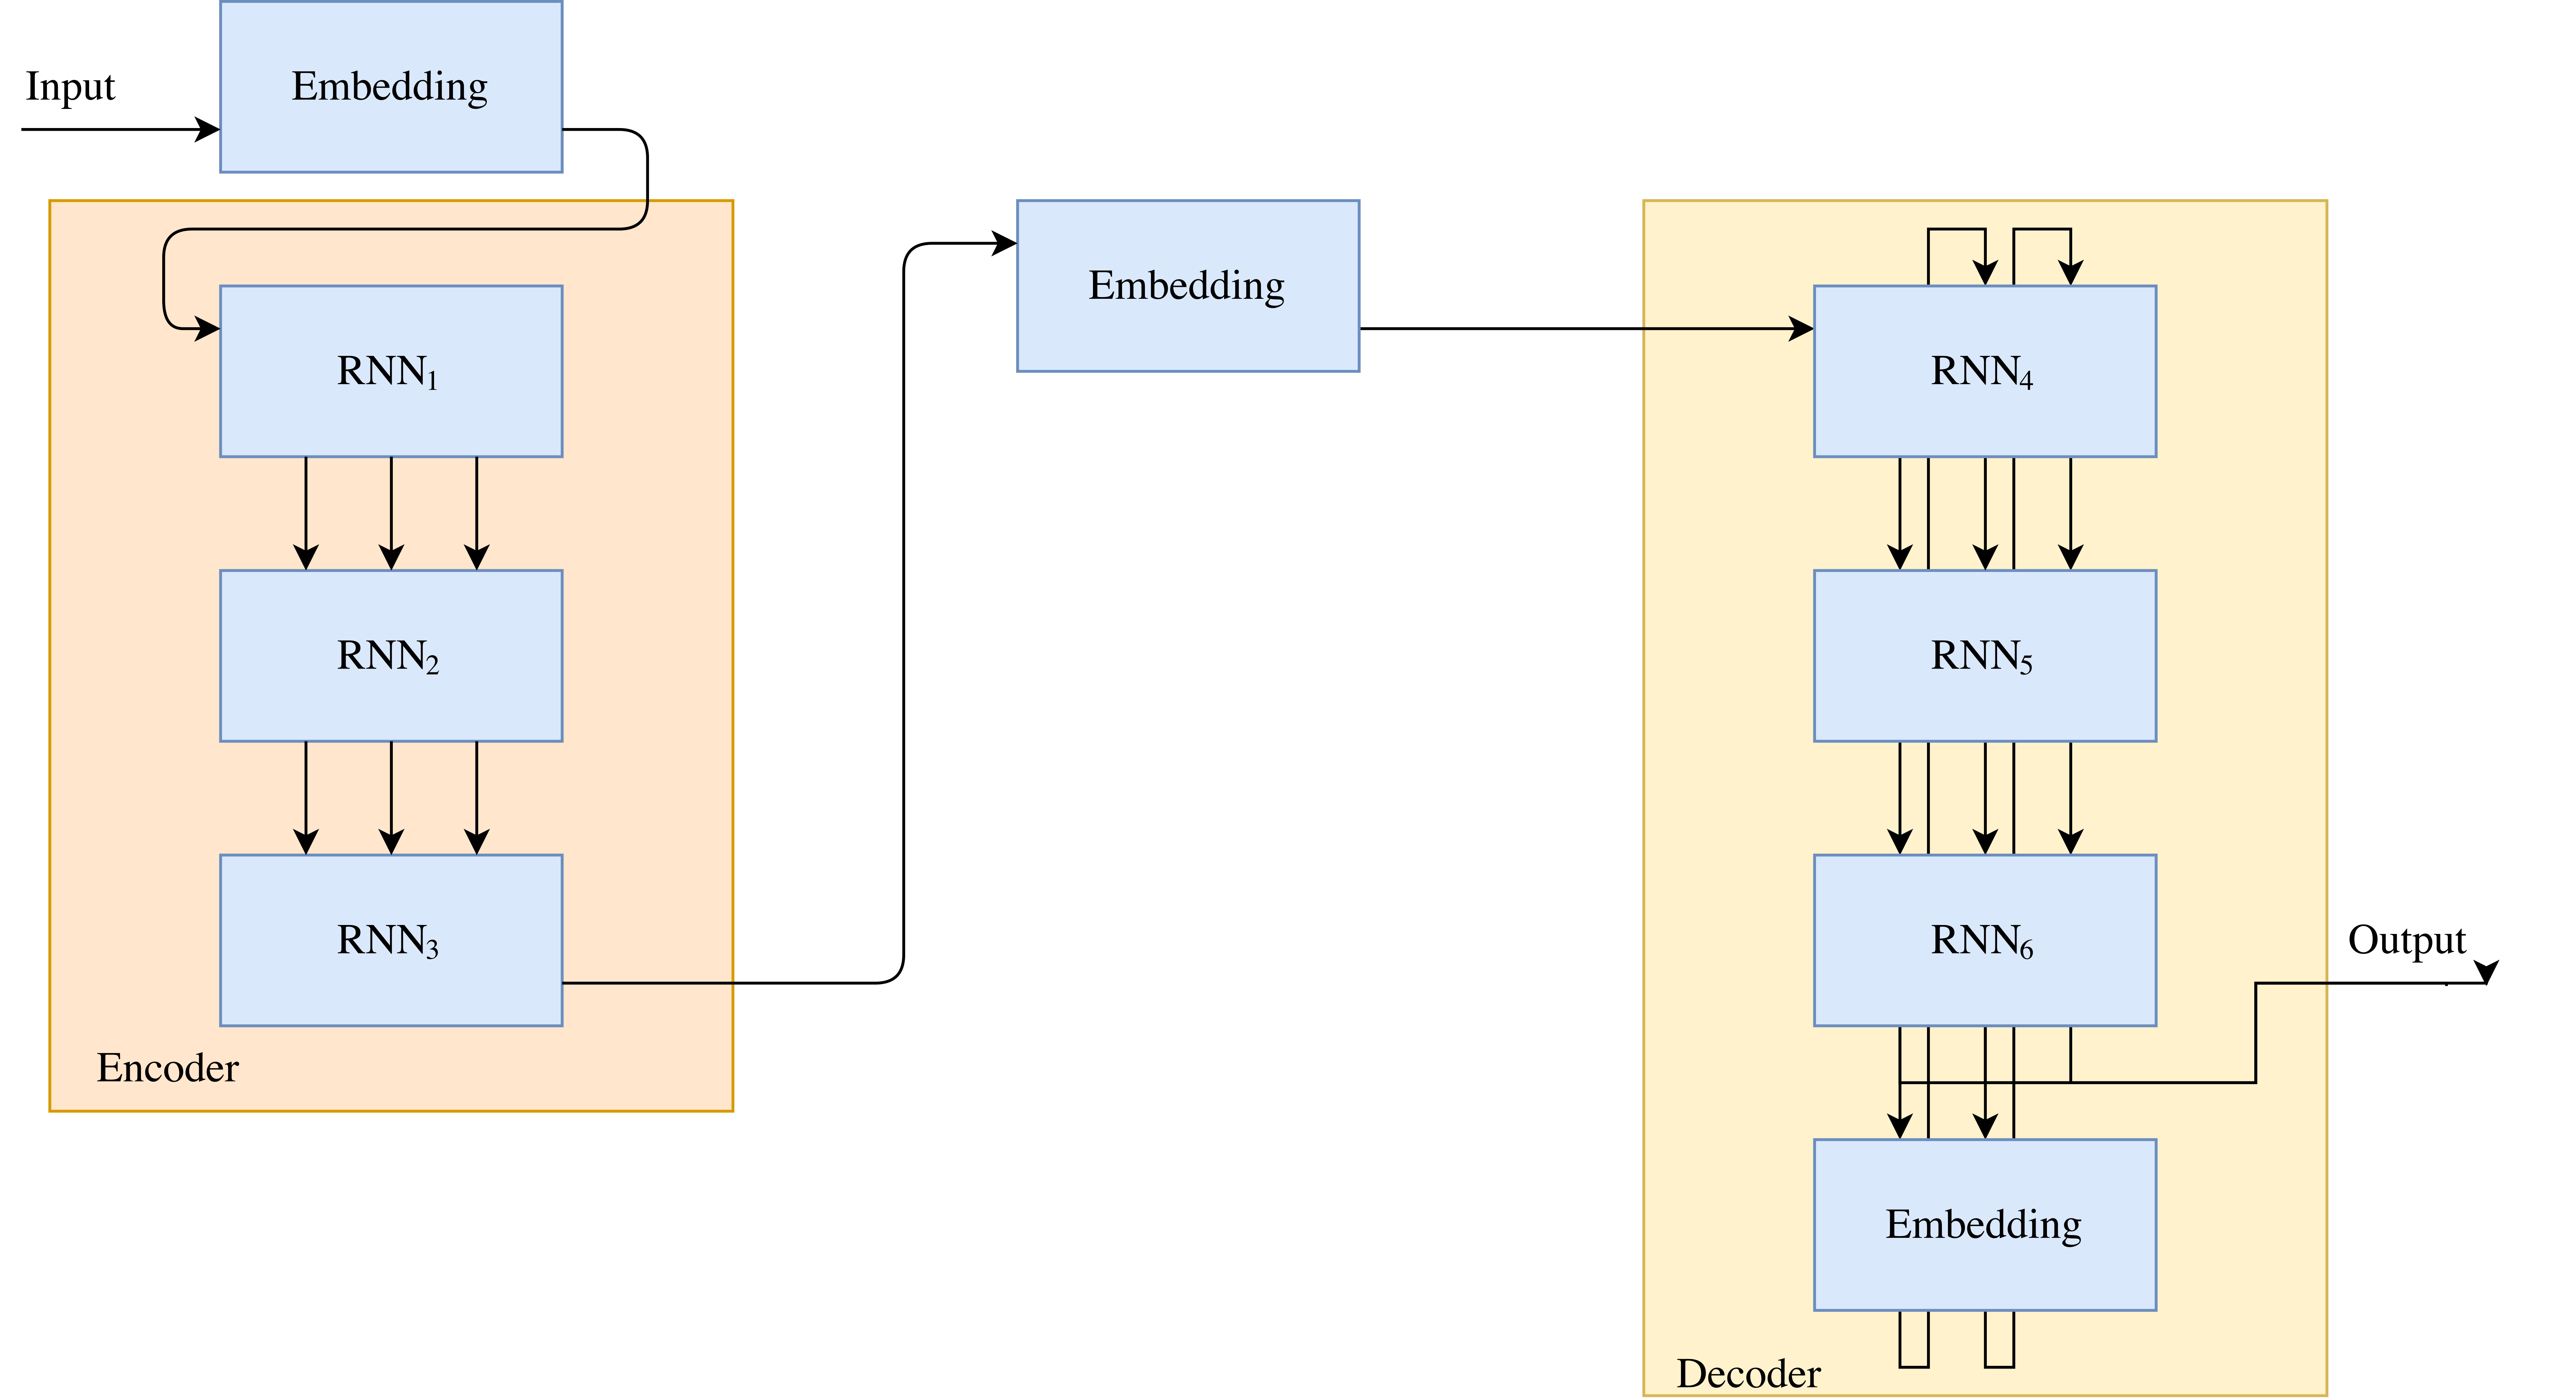
\includegraphics[width=1\textwidth]{fig/models/encdecreg_model.png}
    \caption{Simplified illustration of the {\tt EncDecReg} model}
    \label{fig:encdecreg_model}
\end{figure}

The {\tt EncDecReg} model is illustrated in Figure \ref{fig:encdecreg_model}. The stacked recurrent units are handled differently in this model compared to the {\tt VecRep} model. In the {\tt VecRep} model, each RNN cell iterates all the timesteps in the input and passes its output to the next RNN cell which does the same, whereas in this model the RNNs are called sequentially for each timestep. This means that for every timestep \(T\) the input is first fed to \(\text{RNN}_1\), then \(\text{RNN}_2\), and so on. This results in a cell that consists of multiple layers, whereas {\tt VecRep} has multiple cells in sequence. The last hidden state of the encoder RNN layers is passed as the initial hidden states for the RNN layers in the decoder, illustrated with a dashed line. In the decoder, we both output from \(\text{RNN}_6\), while also passing the output to an embedding layer and feeding it back into the first RNN layer in the cell again. Note that the embedding between the encoder and decoder, and the embedding below the \(\text{RNN}_6\) layer is the same embedding.

%%=========================================

\section{Attention Encoder-Decoder}
\label{sec:attention_encoder_decoder}
The last model also implements the encoder-decoder framework, similarly to the {\tt EncDecReg} model. In addition, this model also implements the attention mechanism, and is named {\tt EncDecAtt} for short. As explained in Section \ref{sec:attention_mechanism}, the attention mechanism allows the decoder to peek into the input by providing a list of values from the input. The implementation of the attention mechanism used in this model is based on \citep{vinyals2015grammar}.

\begin{figure}[!ht]
    \centering
    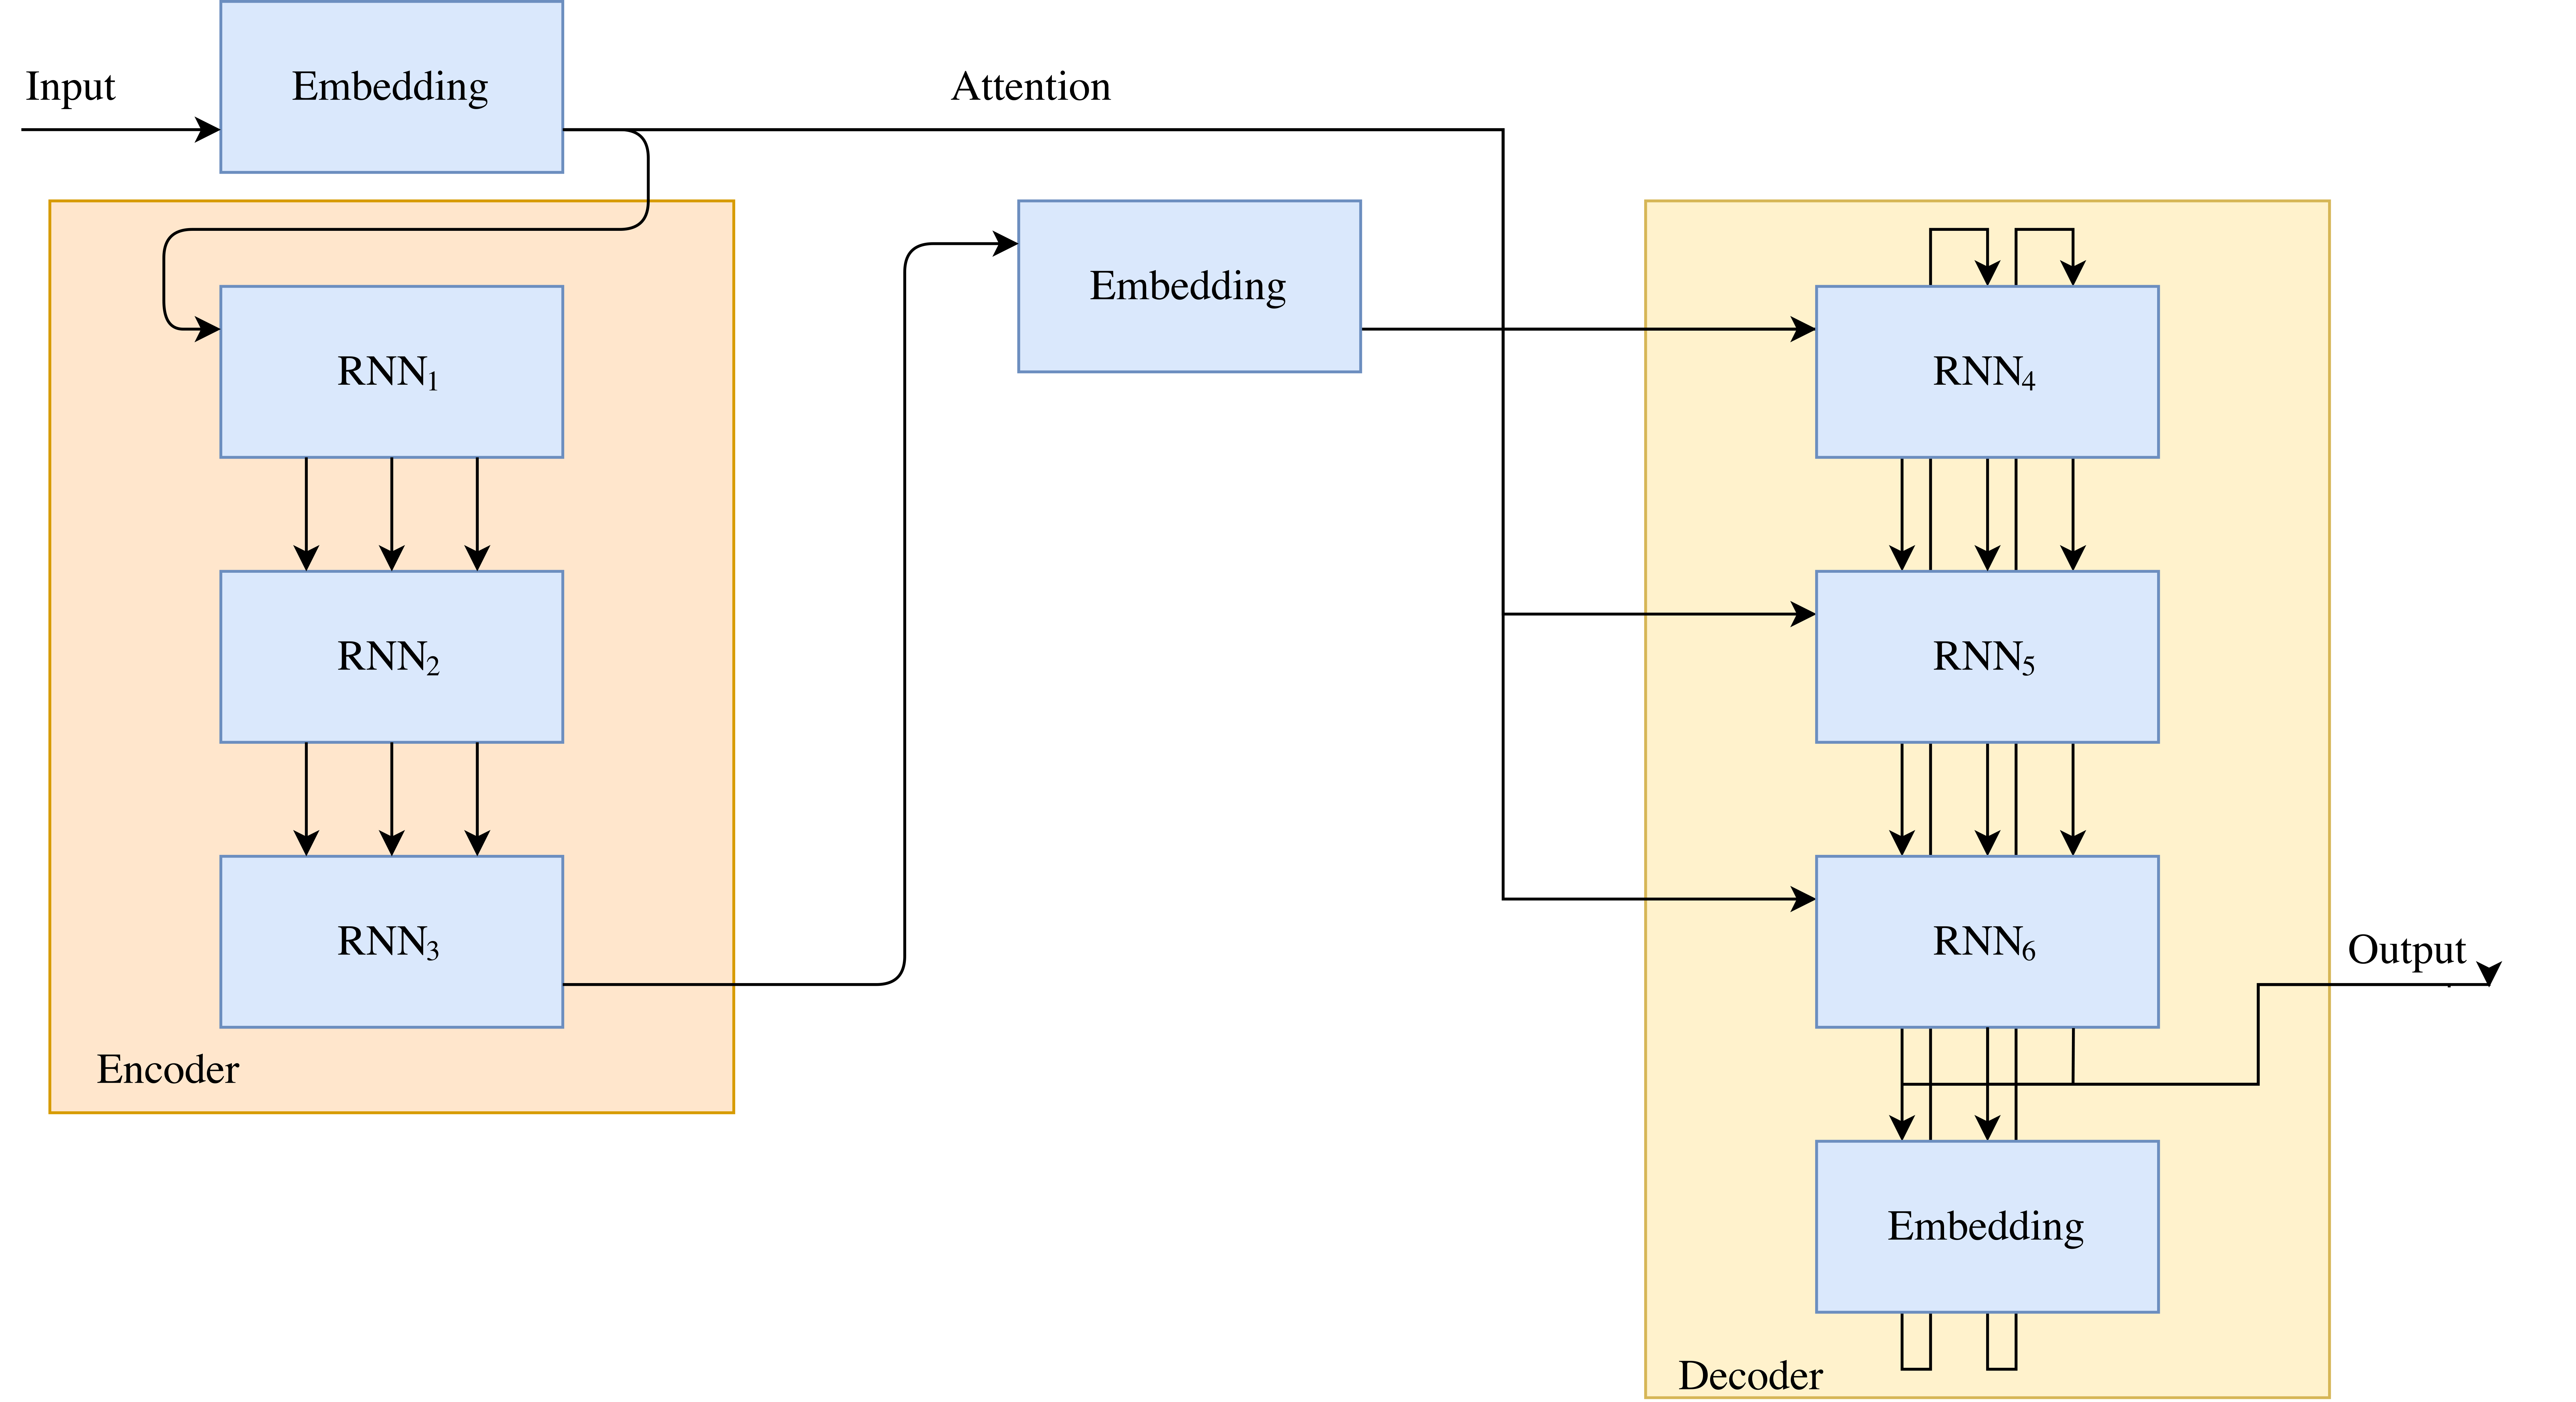
\includegraphics[width=1\textwidth]{fig/models/encdecatt_model.png}
    \caption{Simplified illustration of the {\tt EncDecAtt} model}
    \label{fig:encdecattg_model}
\end{figure}

The {\tt EncDecAtt} model is illustrated in Figure \ref{fig:encdecattg_model}. The difference between this model and the {\tt EncDecReg} model is the additional input for the RNN layers in the decoder cell. This input is fetched directly from the input and allows the attention mechanism to attend to this data, in addition to the hidden states from the encoder cell.